\subsection{Resumen}

Para imágenes suficientemente grandes, donde la cache no es suficiente, los filtros en asm con simd son mucho mas rápidos que los hechos en C

\subsection{Experimentaciones}

Nuestra hipotesis se basa en que asembler consigue un mejor uso de la cache, y le atribuimos a eso su velocidad con respecto a C, para comprobar eso observaremos los miss/hit de las diferentes implementaciones de los filtros. Usaramos imagenes chicas que no tengan problema en entrar en la cache y muy pesadas. El objetivo de esto es ver si cuando la imagen es mas grande que la cache, los miss/hit de la misma cambian mucho o no en comparacion a los de las imagenes chicas, asi como tambien ver estas diferencias entre assembler y C. En este caso haremos tests en una computadora que tiene una cache de 6mb, por lo que usaremos imagenes que tienen un peso superior al de ese valor. \\


Con esto esperamos corroborar que los filtros implementados en assembler con simd tienen mas hit que los de C en situaciones que incluyen tanto a procesar una imagen mas grande que la cache como con una mas chica, y por ende son mucho mas rapidos que los de C. Queremos ver asi, si implementar codigo directamente en asm resulta en un mejor uso de la cache, y entonces concluir que esto es una de las razones de lo rapido que son los filtros en asm con respecto a los de C. A medida que relizamos los experimentos iremos incrementado el tamaño de la imagen para ver si la relacion Miss/Hit de ambos filtros va variando o no. Con cada tamaño de imagen además variaremos los parametros del filtro. \\


Los siguientes experimentos los realizamos sobre el filtro blur, ya que como este es mas complicado, tiene mas ciclos y accede a posiciones de la imagen mas inesperadas que las del filtro diff, consideramos que le exige mas al predictor de saltos, y al no ser lineal el contenido de la cache cambiara con mas frecuencia. De esta manera las diferencias en el uso de cache, si es que las hay, seran más pronunciadas. Este filtro ademas recibe parametros, si bien cambiar sigma no altera el uso de la cache (pues solo afecta cuentas), cambiar el radio produciria que mientras este aumente, se utilice una parte de la imagen mas grande y completamente diferente e inesperada, por eso decidimos hacer las pruebas con este filtro. \\


Para ver los el uso de la cache utilizaremos el programa valgrind y realizaremos cada experimento varias veces para obtener un promedio sacando outliers. Fijamos como 30 el radio maximo ya que si lo incrementamos mas, el valgrind demora demasiado en emular el comportamiento de la cache (mas de media hoa). A continuacion mostraremos algunos resultados obtenidos con las diferentes imagenes, mostrando su peso y porcentaje de miss. \\
Para obtener estos datos usamos la herramienta de Valgrind Cachegrind de la siguiente manera: $valgrind --tool=cachegrind filtro$\\
Las imágenes son las siguientes:\\
2560x1080: 2k.bmp\\
192x1080: 1k.bmp\\
1280x720: sd.bmp\\
1024x600: 600.bmp\\
320x480: 480.bmp\\

\subsection{Datos obtenidos}

\begin{figure}[H]
\begin{center}
%\minipage{0.8\textwidth}
  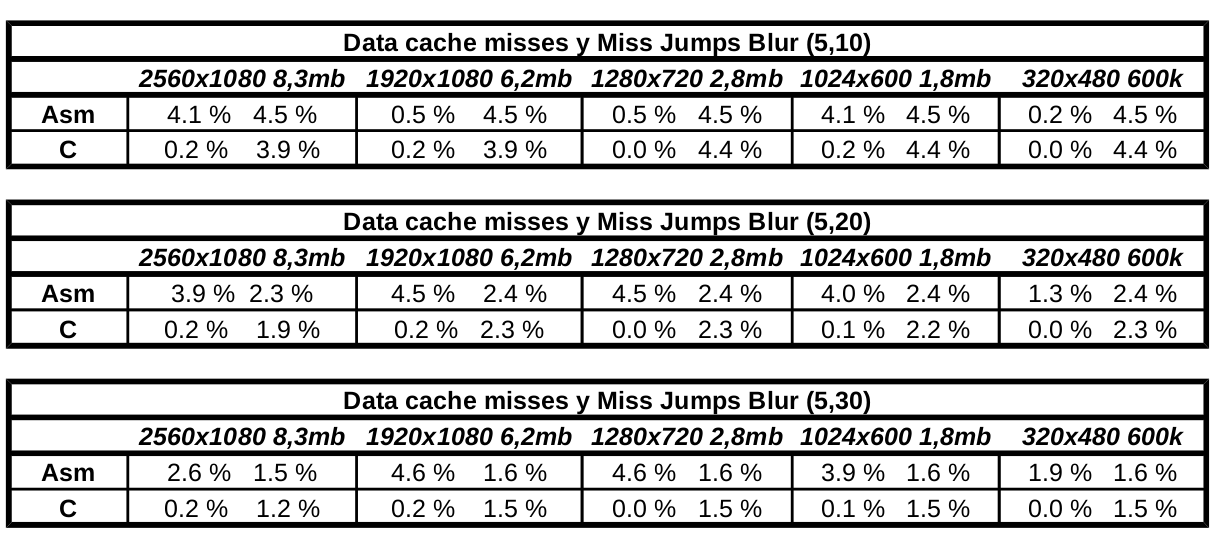
\includegraphics[width=\linewidth]{cache/tabla.png}
%\endminipage
\end{center}
\end{figure}

\subsection{Gráficos} 


\begin{figure}[H]
\begin{center}
%\minipage{0.8\textwidth}
  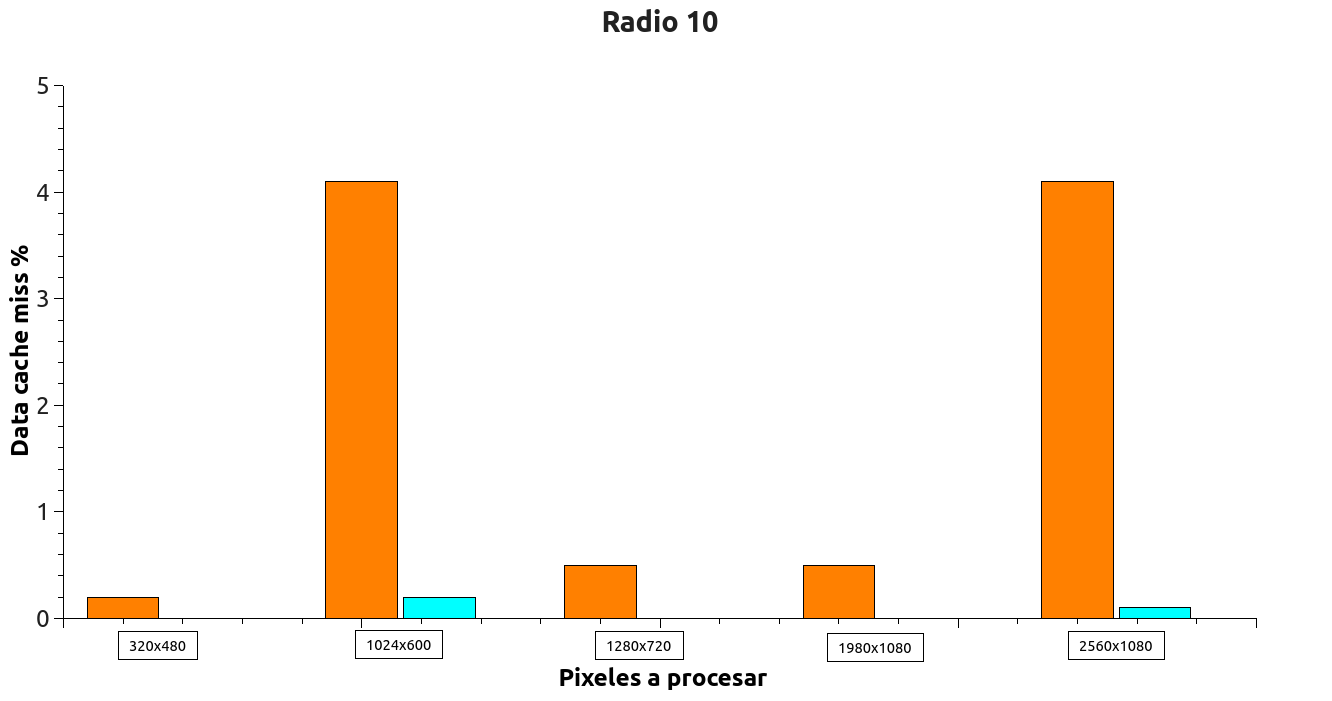
\includegraphics[width=\linewidth]{cache/Radio10.png}
  %\endminipage
\end{center}
\end{figure}

\begin{figure}[H]
\begin{center}
%\minipage{0.8\textwidth}
  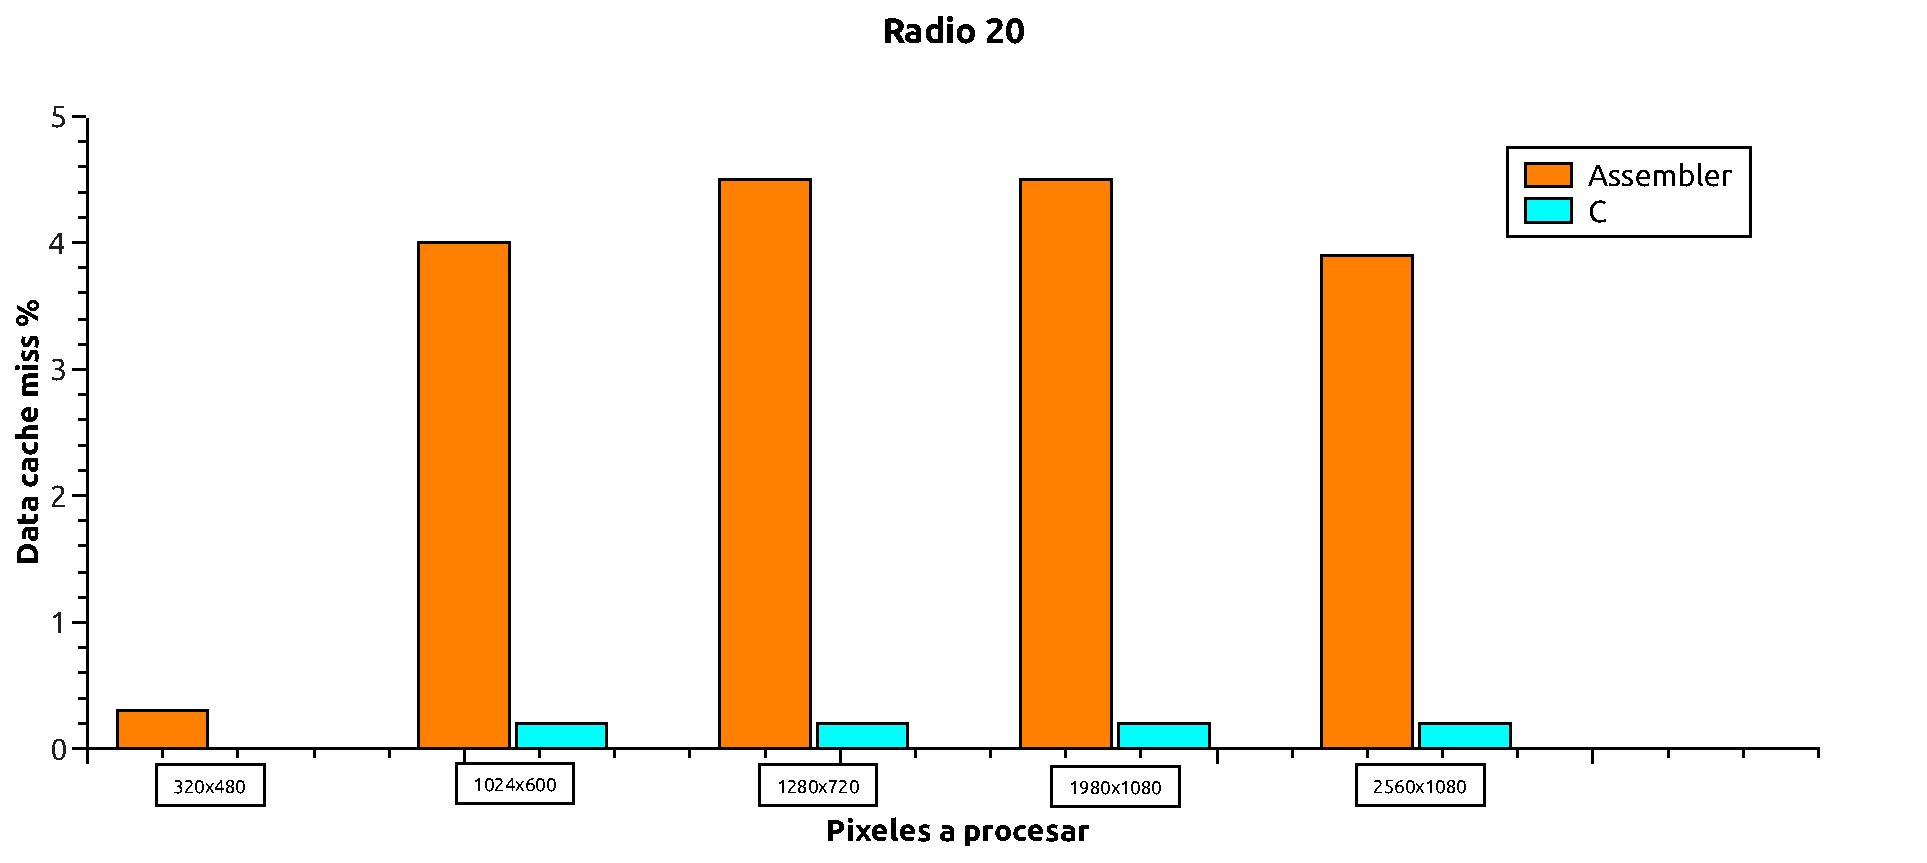
\includegraphics[width=\linewidth]{cache/Radio20.pdf} 
%\endminipage  
\end{center}
\end{figure}

\begin{figure}[H]
\begin{center}
%\minipage{0.8\textwidth}
  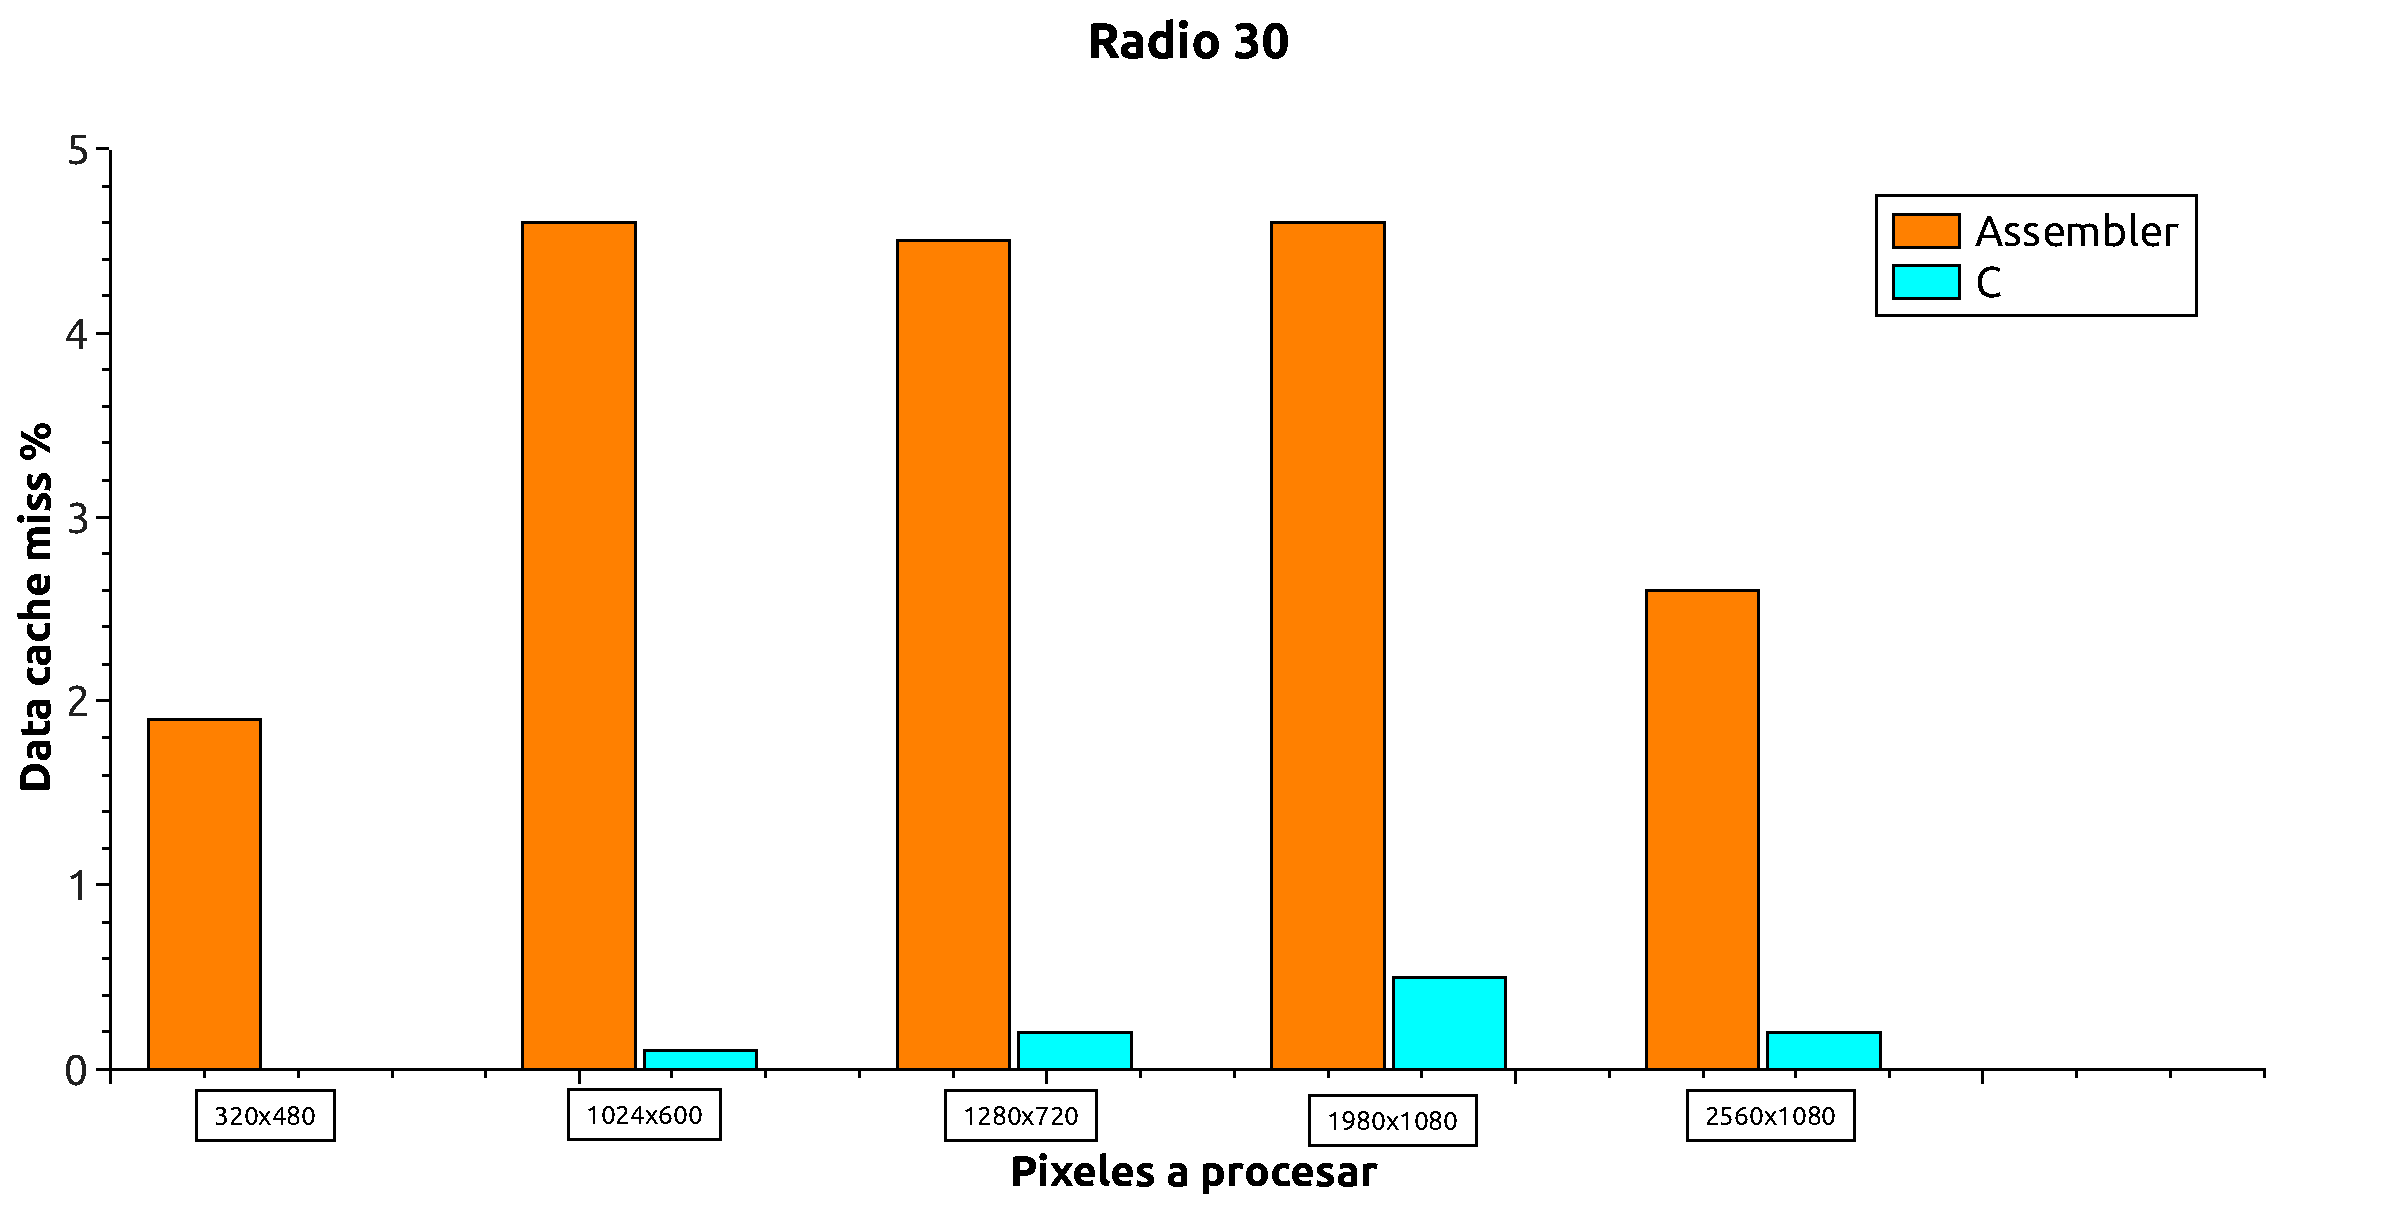
\includegraphics[width=\linewidth]{cache/Radio30.pdf}
  %\endminipage
\end{center}
\end{figure}

\subsection{Conclusion} 

A partir de los gráficos y de los datos obtenidos se puede ver claramente un mejor uso de la cache por parte de los filtros en C, esto va en contra de nuestra hipotesis. Sin embargo conlcuimos que esto pasa porque el compilador hace un muy buen trabajo a la hora de pasar el Código en C a lenguaje de máquina y que lo hace de una manera que aprovecha al máximo el uso la cache. Esta conclusión sale de que al ver el porcentaje de miss de los filtros en C a medida que aumentamos el radio y el tamaño de la imagen es siempre muy similar. Por lo tanto el tamaño de imagen y el radio no afectan el radio miss/hit de la cache en el filtro implementado en  C. Esto no pasa con nuestros filtros en asm, en los cuales si se puden ver variaciones mas notables en el porcentaje de miss. De esto conlcuimos que el problema de los miss en asm es la forma en que programamos el filtro. \\
Por otro lado notamos que si bien el porcentaje de miss jumps de ambas implementaciones es muy similar, la cantidad de saltos que realiza C es muchisimo mas alta que la de asm. No inclumos estos numeros en el infome porque con un radio de 20 valgrind no terminaba de procesar la imagen, sin embargo al parar la emulacion de la cache en diferentes momentos, el porcentaje de miss era siempre el mismo, tanto en asm como en C. Con radios mas chicos la emulacion si terminaba y si se podia observar una cantidad de saltos hasta 5 veces mayor en la implementacion de C. Esto se puede atribuir a que asm utiliza simd y procesa 4 pixeles por iteracion y por ende realiza menos viajes a la memoria, y por eso es mas rápido.
